\section{Unsere Galaxis}
(=Milchstraße=$\lambda\alpha\lambda\alpha\xi$i$\zeta$)
\subsection{Struktur der Galaxis}
\begin{figure}[H]
	\centering
	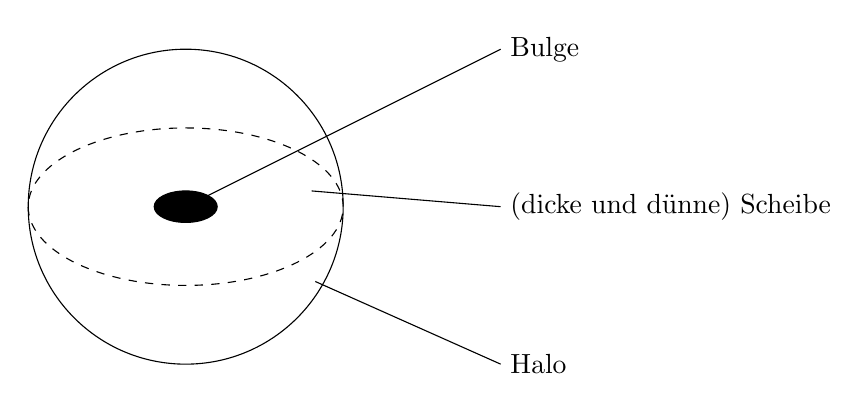
\begin{tikzpicture}[scale=2]
		\draw[fill=black] (0,0)ellipse(0.2cm and 0.1 cm);
		\draw[dashed] (0,0)ellipse(1 cm and 0.5 cm);
		\draw (0,0)ellipse(1cm and 1cm);
		\draw (0,0)--(2,1)node[right]{Bulge};
		\draw (0.8,0.1)--(2,0)node[right]{(dicke und dünne) Scheibe};
		\draw ({0.95*cos(330)},{0.95*sin(330)})--(2,-1)node[right]{Halo};
	\end{tikzpicture}
\end{figure}
\begin{itemize}
	\item stellare Populationen:\\
		Population I (Pop I): Sterne mit Metallizität $Z\sim\num{0.02}\sim Z_\odot$ v.a. in der dünnen Scheibe\\
		Population II (Pop II): metallarm $Z\sim\num{0.001}$ v.a. in der dicken Scheibe, aber auch im Halo und im Bulge
	\item Metallizität und Alter:
		\begin{itemize}[label=$\cdot$]
			\item extrem alte Sterne: $\left[\frac{\text{Fe}}{\text{H}}\right]=-\num{4.5}$
			\item dicke Scheibe: $\left[\frac{\text{Fe}}{\text{H}}\right]=-\num{6.5}$
			\item dünne Scheibe: $\left[\frac{\text{Fe}}{\text{H}}\right]=-\num{0.5}$
			\item sehr junge Sterne: $\left[\frac{\text{Fe}}{\text{H}}\right]=\num{1}$
		\end{itemize}
	\item Hauptursache für die Metallanreicherung im interstellaren Medium: Supernovae!\\
		\underline{Supernova (SN)}: Sternenexplosion mit hoher Leuchtkraft $L\sim 10^9\cdot L_\odot$ (vergleichbar mit $L_B$ einer ganzen Galaxie)
	\item historische Klassifizierung anhand der spektralen Eigenschaften:
		\begin{itemize}
			\item[SN I] keine Balmerlinien des Wasserstoffs
				\begin{itemize}
					\item[SNIa] starkes SiII Emission, $\lambda=\SI{615}{n\m}$
					\item[SNIb,Ic] keine SiII Emission
				\end{itemize}
			\item[SN II] mit Balmerlinien
		\end{itemize}
	\item heute bekannt:
		\begin{enumerate}[label={$(\roman*)$}]
			\item SNII,SNIb,c: Sternenexplosion mit $M_\ast\gtrapprox 8M_\odot$ abgestrahlte Energie $\sim$ $\SI{3e53}{\erg}$ (Neutrinos!)\\
				1. (?) Nachweis von $\num{10}$ Neutrinos der SN1987A
				\begin{itemize}[label={$\to$}]
					\item Wechselwirkung zw. Neutrinus und Sternmaterie (hohe Dichte!)
						\begin{itemize}[label={$\Rightarrow$}]
							\item Explosion der Sternhülle mit $E_\text{kin}\sim 10^{51}\si{\erg}=\SI{1}{\text{foe}}=\SI{1}{\text{Bethe}}$
							\item $10^{49}~\si{\erg}$ umgesetzt in Photonen (nur Bruchteil der Gesamtenergie!)
						\end{itemize}
				\end{itemize}
			\item SNIa: Explosion eines weißen Zerges eines Doppelsternsystems
				\begin{figure}[H]
					\begin{multicols}{2}
						\begin{figure}[H]
							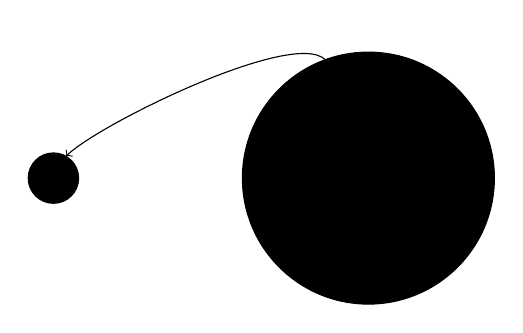
\begin{tikzpicture}[scale=0.8]
								\def\k{5}
								\draw[fill=black] (0,0)circle(0.4cm);
								\draw[fill=black] (\k,0)circle(2 cm);
								\draw[->] ({2*cos(110)+\k},{2*sin(110)}) .. controls +(-0.5,0.5) and +(0.5,0.5) .. ({0.4*cos(60)},{0.4*sin(60)});
							\end{tikzpicture}
						\end{figure}\columnbreak
						Massentransfer (Akkrektion) von seinem Begleiter, bis die Chandrasekhar-Masse $M_{Ch}\approx\SI{1.44}{\sm}$ überschritten wird $\Rightarrow$ SNIa
					\end{multicols}
				\end{figure}
				\begin{itemize}[label={$\to$}]
					\item homogene Anfangsbedingungen für SNIa mit etwa gleicher Leuchtkraft
						\begin{itemize}
							\item[$\Rightarrow$] \textbf{Standardkerzen, die weithin sichtbar sind}
						\end{itemize}
				\end{itemize}
		\end{enumerate}
		\begin{table}[H]
			\def\k{1.5}
			\begin{tabular}{p{2 cm}|p{\k cm}|p{\k cm}|p{\k cm}|p{\k cm}|p{\k cm}|p{\k cm}}
				& neutrales Gas & dünne Scheibe & dicke Scheibe & Bulge & stellarer Halo & DM Halo \\\hline
				$\frac{M}{10^{10}~\si{\sm}}$ & $\num{0.5}$ & $\num{6}$ & $\num{0.2}-\num{0.4}$ & $\num{1}$ & $\num{0.15}$ & - \\\hline
				$\frac{L_B}{10^{10}~\si{\sl}}$ & - & $\num{1.8}$ & $\num{0.02}$ & $\num{0.3}$ & $\num{0.1}$ & $\num{0}$ \\\hline
				$\frac{\frac{M}{L_B}}{\frac{M_\odot}{L_\odot}}$ & - & $\num{3}$ & $\num{10}$ & $\num{3}$ & $\sim\num{1}$ & - \\\hline
				Durch- messer ($\si{k\pc}$) & $\num{50}$ & $\num{50}$ & $\num{50}$ & $\num{2}$ & $\num{100}$ & $>\num{200}$\\\hline
				Form & $e^{-\frac{z}{h_z}}$ & $e^{-\frac{z}{h_z}}$ & $e^{-\frac{z}{h_z}}$ & Balken? & $r^{-3.5}$ & $\frac{1}{w^2+r^2}$ \\\hline
				Skalenhöhe $h_z$ ($\si{k\pc}$) & $\num{0.13}$ & $\num{0.325}$ & $\num{1.5}$ & $\num{0.4}$ & $\num{3}$ & $\num{2.8}$ \\\hline
				Geschwindig- keitsdispersion $\si{k\m\per\s}$& $\num{7}$ & $\num{20}$ & $\num{40}$ & $\num{120}$ & $\num{100}$ & - \\\hline
				$\left[\frac{\text{Fe}}{\text{H}}\right]$ & $>\num{0.1}$ & $-\num{0.5}-(+\num{0.3})$ & $(-\num{1.6})-(-\num{0.4})$ & $-\num{1}-(-\num{1})$ & $-\num{4.5}-(-\num{0.5})$ & - \\
			\end{tabular}
		\end{table}
\end{itemize}
\subsection{Kinematik der Galaxis}
\begin{figure}[H]
	\begin{tikzpicture}[scale=2]
		\draw (0,0)ellipse(2cm and 0.8cm);
		\draw[white,fill=white] (-2,0)--(2,0)--(2,1)--(-2,1)--cycle;
		\draw (-2,0)--(-2,1)(2,0)--(2,1);
		\draw (0,1)ellipse(2cm and 0.8cm);
		\coordinate (x) at (0,1);
		\node at (x){$\times$};
		\node[name=r1] at (0.9,1.5){};
		\node[name=r2] at (1.5,1.4){};
		\node[name=r3] at (1.9,1.1){};
		\draw (x)--(3,2)node[right]{galaktisches Zentrum};
		\draw[->] (r1) .. controls (r2) and (r2) .. (r3)node[midway,name=r]{};
		\draw (r)--(3,1.5)node[right]{Rotation};
		\draw[->] (x)--(0,2)node[above]{$z$};
		\draw (-1.5,0.9)circle(0.1 cm)coordinate(s);
		\draw (s)--(-0.9,1.25)coordinate(f);
		\coordinate (a) at ([yshift=0.25 cm]f);
		\node at (a){$\ast$};
		\draw (s)--(x);
		\draw (f)--(x);
		\pic[draw,"$l$",angle eccentricity=1.5] {angle=x--s--f};
		\pic[draw,"$\theta$",angle eccentricity=1.5] {angle=f--x--s};
		\draw[dashed] (a)--([yshift=0.25cm]x)(a)--(f)(a)--(s);
	\end{tikzpicture}
\end{figure}
\begin{itemize}
	\item sphärische Galaktische Koordinaten $(l,b)$ mit der Sonne als Zentrom: $l=$ galaktische Länge, $b=$ galaktische Breite $b=\SI{90}{\degree}\hat{=}$ galaktischer Nordpol (NGP)
	\item zylindrische Galaktische Koordinaten $(R,\theta,z)$ mit Geschwindkigkeitskomponenten $(U,V,W)$
	\item Körper mit der Bahnkurve $(R(t),\theta(t),z(t))$ hat die Geschwindigkeitskomponenten:
		\begin{equation*}
			U=\frac{dR}{dt};\quad V=R\cdot\frac{d\theta}{dt};\quad W=\frac{dz}{dt}
		\end{equation*}
	\item fiktives Ruhesystem: Local Standard of Rest (LSR) mit $U_\text{LSR}=0$, $V_\text{LSR}=0$, $W_\text{LSR}=0$\\
		wobei $v_0=V(R_0)$ Kreisbahngeschwindigkeit am Ort der Sonne entspricht
	\item Pekuliargeschwindigkeit (=Geschwindigkeit relativ zum LSR):
		\begin{equation*}
			\vec{v}=(u,v,w)=(U-U_\text{LSR},V-V_\text{LSR},W-W_\text{LSR})=(U,V-V_0,W)
		\end{equation*}
		$\vec{v}_\odot$: Sonnenbewegung relativ zum LSR
		\begin{itemize}
			\item $\vec{v}=\vec{v}_\odot+\underset{\text{Geschwindigkeit eines Sterns relativ zur Sonne}}{\underset{\uparrow}{\Delta\vec{v}}}$
		\end{itemize}
	\item Mittelwert der Pekuliargeschwindigkeitskomponenten:
		\begin{equation*}
			\langle u\rangle=0,\langle w\rangle=0,\langle v\rangle\neq 0
		\end{equation*}
		$\langle v\rangle = -C\cdot \langle u^2\rangle$
		\begin{equation*}
			\Rightarrow \vec{v}_\odot = (-\langle\Delta u\rangle , (-C\cdot\langle u^2\rangle -\langle\Delta v\rangle),-\langle\Delta w\rangle)
		\end{equation*}
	\item Wie kann $C$ gefunden werden? $\Rightarrow$ Messen von $\langle\Delta v\rangle$ und $\langle u^2\rangle$ von verschiedenen Sternpopulationen
		\begin{figure}[H]
			\begin{multicols}{2}
				\begin{tikzpicture}
					\draw[->] (-0.1,0)--(2,0)node[below right]{$\langle u^2\rangle$};
					\draw[->] (0,-0.1)--(0,2)node[above left]{$\langle\Delta v\rangle$};
					\draw (-0.1,1.5)--(0.1,1.5)node[right]{0};
					\draw (0,1)--(1.5,0.25);
					\draw[<->,xshift=-0.1 cm] (0,1)--(0,1.5)node[midway,left]{$\vec{v}_\odot$};
				\end{tikzpicture}\columnbreak
				\begin{equation*}
					\vec{v}_\odot=(-10,7,5)\si{\km\per\s}
				\end{equation*}
			\end{multicols}
		\end{figure}
	\item Asymmetrischer Drift:
		\begin{figure}[H]
			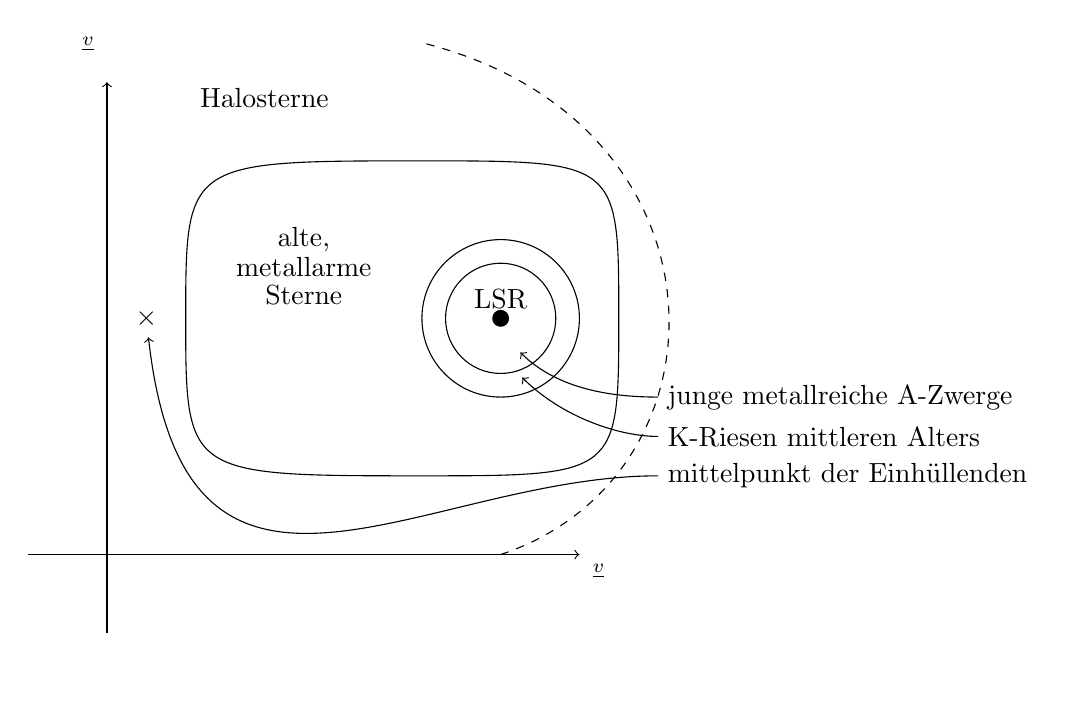
\begin{tikzpicture}
				\draw[->] (-1,0)--(6,0)node[below right]{$\frac{v}{\si{\frac{\km}{\s}}}$};
				\draw[->] (0,-1)--(0,6)node[above left]{$\frac{v}{\si{\frac{\km}{\s}}}$};
				\draw[fill=black] (5,3)circle(0.1cm)node[name=lsr,above]{LSR};
				\draw (5,3)circle(0.7 cm);
				\draw[->] (7,2)node[right]{junge metallreiche A-Zwerge} .. controls +(-0.5,0) and +(0.5,-0.5) .. ({5+0.5*cos(300)},{3+0.5*sin(300)});
				\draw (5,3)circle(1cm);
				\draw[->] (7,1.5)node[right]{K-Riesen mittleren Alters} .. controls +(-0.5,0) and +(0.5,-0.5) .. ({5+0.8*cos(290)},{3+0.8*sin(290)});
				\draw (4,5) .. controls (1,5) and (1,5) .. (1,3) .. controls (1,1) and (1,1) .. (4,1) .. controls (6.5,1) and (6.5,1) .. (6.5,3) .. controls (6.5,5) and (6.5,5) .. cycle;
				\node at (2.5,4){alte,};
				\node at (2.5,3.65){metallarme};
				\node at (2.5,3.3){Sterne};
				\draw[dashed] (5,0) .. controls +(3,1) and +(4,-1) .. (4,6.5);
				\node[name=x] at (0.5,3){$\times$};
				\draw[->] (7,1)node[right]{mittelpunkt der Einhüllenden} .. controls +(-3,0) and +(0.5,-4.5) .. (x);
				\node at (2,5.8){Halosterne};
			\end{tikzpicture}
		\end{figure}
		\begin{itemize}[label={$\cdot$}]
			\item $(u,v)$-Verteilung junger Sterne eng um $u=v=0$, die für ältere Sterne breiter wird (Dispersion wg. Gravitationswechselwirkungen)
			\item $v\approx -\SI{220}{\frac{\km}{\s}}$ Mittelpunkt der kreisförmigen Einhüllenden der Halopopulation (mit der älteren Sterne)
			\item Annahme: Halo rotiert nicht (oder nur langsam) $\Rightarrow V_0=V(R_0)=\SI{220}{\frac{\km}{\s}}$
		\end{itemize}
	\item GG-Bedingung für eine Kreisbahn: Zentrifugalkraft=Gravitationskraft
		\begin{align*}
			\Leftrightarrow \frac{mV^2}{R}&=G\frac{mM}{R^2} \text{ mit } M=M(R)=\text{ Masse im Inneren der Kugelschale}\\
			\Rightarrow M(R_0)&=\frac{V_0^2R_0}{G}=\SI{8.8e10}{\sm}
		\end{align*}
		\begin{itemize}
			\item Umlaufzeit des LSR um die Galaxis:
				\begin{equation*}
					P=\frac{2\pi R_0}{V}=\SI{230e6}{a}
				\end{equation*}
		\end{itemize}
\end{itemize}
